
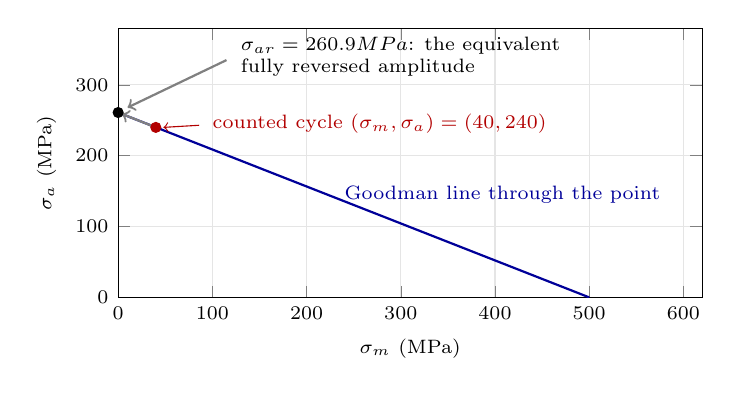
\begin{tikzpicture}
\begin{axis}[width=9.0cm,height=5.0cm,xlabel={$\sigma_m$ (MPa)},ylabel={$\sigma_a$ (MPa)},
 xmin=0,xmax=620,ymin=0,ymax=380,grid=both,grid style={gray!20},
 label style={font=\scriptsize},tick label style={font=\scriptsize}]
\addplot[thick,blue!60!black,domain=0:500,samples=2]{261*(1-x/500)};
\node[font=\scriptsize,blue!60!black,anchor=west] at (axis cs:230,145) {Goodman line through the point};
\addplot[only marks,mark=*,mark size=1.8pt,red!70!black] coordinates {(40,240)};
\node[font=\scriptsize,red!70!black,anchor=west] at (axis cs:90,245) {counted cycle $(\sigma_m,\sigma_a)=(40,240)$};
\draw[->,red!70!black] (axis cs:86,243) -- (axis cs:48,240);
\addplot[only marks,mark=*,mark size=1.8pt,black] coordinates {(0,261)};
\node[font=\scriptsize,anchor=west,align=left] at (axis cs:120,340) {$\sigma_{ar}=\SI{260.9}{MPa}$: the equivalent\\ fully reversed amplitude};
\draw[->,thick,gray] (axis cs:115,335) -- (axis cs:10,268);
\draw[->,thick,gray] (axis cs:40,240) -- (axis cs:4,259);
\end{axis}
\end{tikzpicture}
